
\section{Getting started}\label{sec:start}\index{PISM!getting started}

\subsection{Installing PISM}

To install PISM, see the \,\emph{Getting PISM}\, tab at \href{http://www.pism-docs.org}{\texttt{www.pism-docs.org}}.  Or use the PISM Installation Manual (PDF).\footnote{At \url{http://www.pism-docs.org/wiki/lib/exe/fetch.php?media=installation.pdf}.}

Once installed, the executable \texttt{pismr} should be available on your system's ``path''; confirm this with ``\texttt{which pismr}''.  The instructions below also assume you are using a \texttt{bash} shell or one that accepts \texttt{bash} syntax.  The examples below assume you have the PISM source code in the directory ``\texttt{pism/}''.

\subsection{A Greenland ice sheet example}

We get started with an extended example showing how to generate initial states for prognostic model experiments on the Greenland ice sheet.  Ice sheet and glacier model studies often involve modeling present and past states using actions like the ones demonstrated in this section.  The particular choices made here are motivated by the evaluation of initialization methods in \cite{AschwandenAdalgeirsdottirKhroulev}.

We use data assembled by the \href{http://websrv.cs.umt.edu/isis/index.php/SeaRISE_Assessment}{Sea-level Response to Ice Sheet Evolution (SeaRISE)} group \cite{Bindschadler2013SeaRISE}.  SeaRISE was a community-organized assessment process providing an upper bound on ice sheet contributions to sea level in the next 100--200 years, especially for the IPCC AR5 report in 2013.

This example is a hands-on first look at PISM.  It is not an in-depth tutorial, and some details of what is happening will only be explained later.  The remainder of this manual lists PISM options, discusses nontrivial modeling choices, and explains the ways users may need to preprocess input data.

Some of the PISM output figures in this section were produced using a supercomputer.  Though the basic run here, on a rather coarse $20\,\textrm{km}$ grid, can be done on a typical workstation or laptop, PISM is designed to make high resolution possible by exploiting large-scale parallel processing \cite[among many other examples]{AschwandenAdalgeirsdottirKhroulev,Golledgeetal2012,Golledgeetal2013}.


\subsection{Input data for the Greenland ice sheet}

The NetCDF data used to initialize SeaRISE runs is freely-available online: 
\medskip

\centerline{\protect{\textbf{\url{http://websrv.cs.umt.edu/isis/index.php/Present_Day_Greenland}}}}
\medskip

\noindent The quickest way to get the file is to do
\begin{verbatim}
$ cd pism/examples/std-greenland
$ ./preprocess.sh
\end{verbatim}
\noindent The script \texttt{preprocess.sh} requires \texttt{wget} and also the NetCDF Operators (``NCO''; \url{http://nco.sourceforge.net/}).  It downloads the version 1.1 of the SeaRISE ``master'' present-day data set, which contains ice thickness and bedrock topography from BEDMAP \cite{BamberLayberryGogenini}, and modeled precipitation rates from RACMO \cite{Ettemaetal2009}, among other fields.

In particular, it creates three new NetCDF files which can be read by PISM.  The spatially-varying fields from the downloaded ``master'' file, with adjusted metadata, go in the PISM-readable file \texttt{pism_Greenland_5km_v1.1.nc}.  The other two new files contain famous time-dependent paleo-climate records from ice core and seabed core records; \texttt{pism_dT.nc} has GRIP \cite{JohnsenetalGRIP} while \texttt{pism_dSL.nc} has SPECMAP \cite{Imbrieetal1984}.

Any of these NetCDF files can be viewed with \texttt{ncview} or other NetCDF visualization tools; see Table \ref{tab:NetCDFview} below.  An application of IDV to the master data set produced Figure \ref{fig:sr-input}, for example.  Use \texttt{ncdump -h} to see the metadata and history of the files.

\begin{figure}[ht]
\centering
\mbox{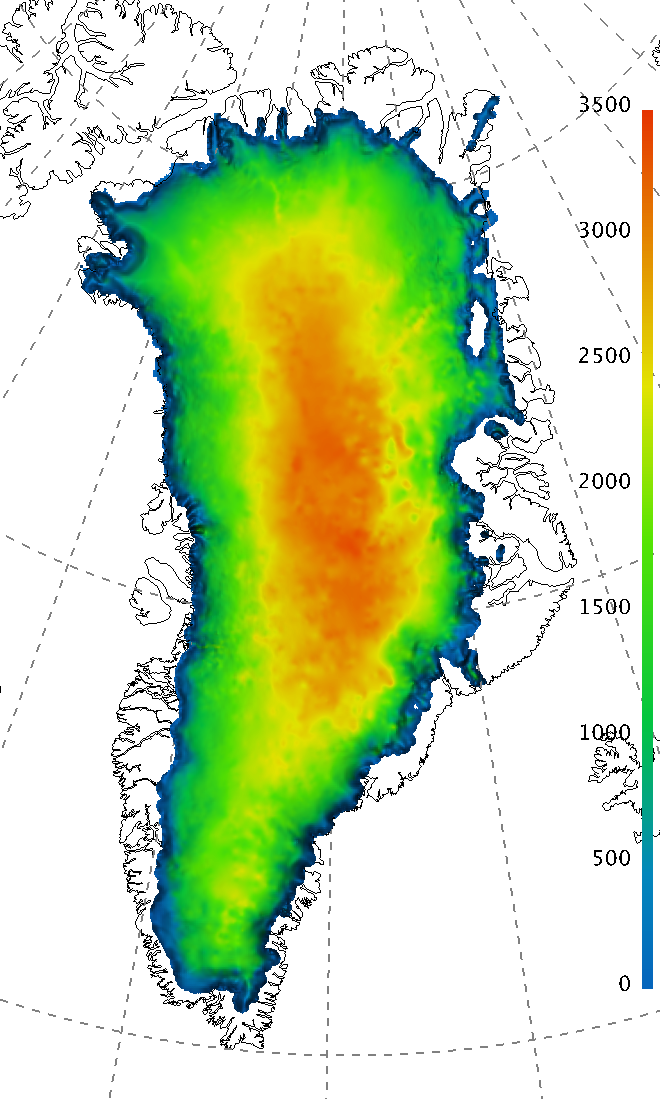
\includegraphics[width=2.0in,keepaspectratio=true]{sr-greenland-thk}
  \qquad
  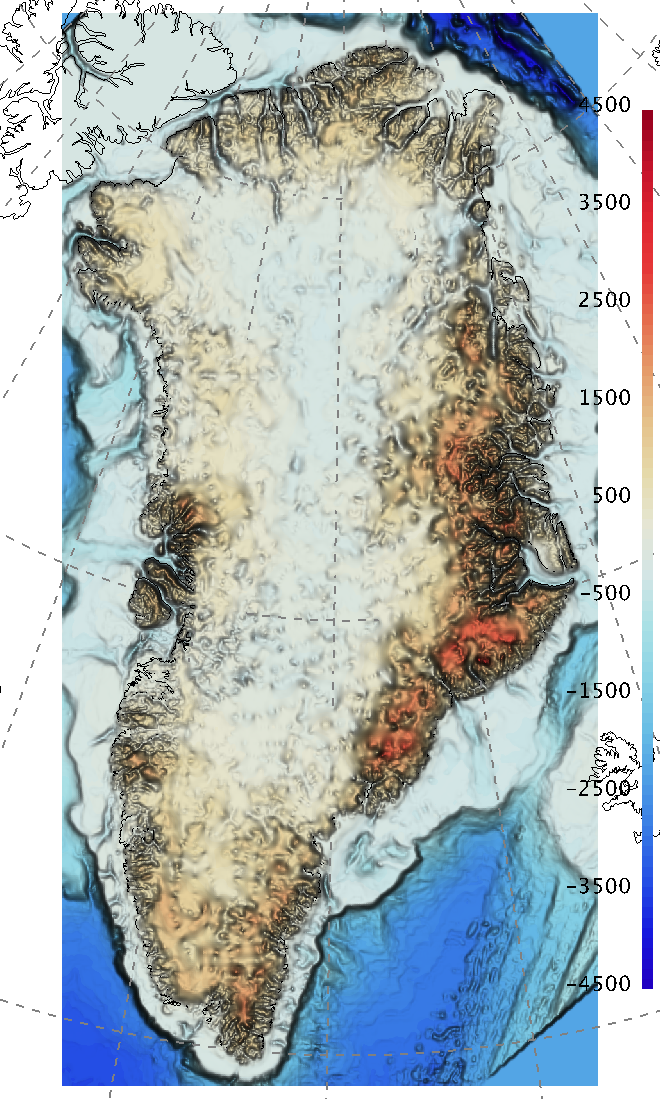
\includegraphics[width=2.0in,keepaspectratio=true]{sr-greenland-topg}
  \qquad
  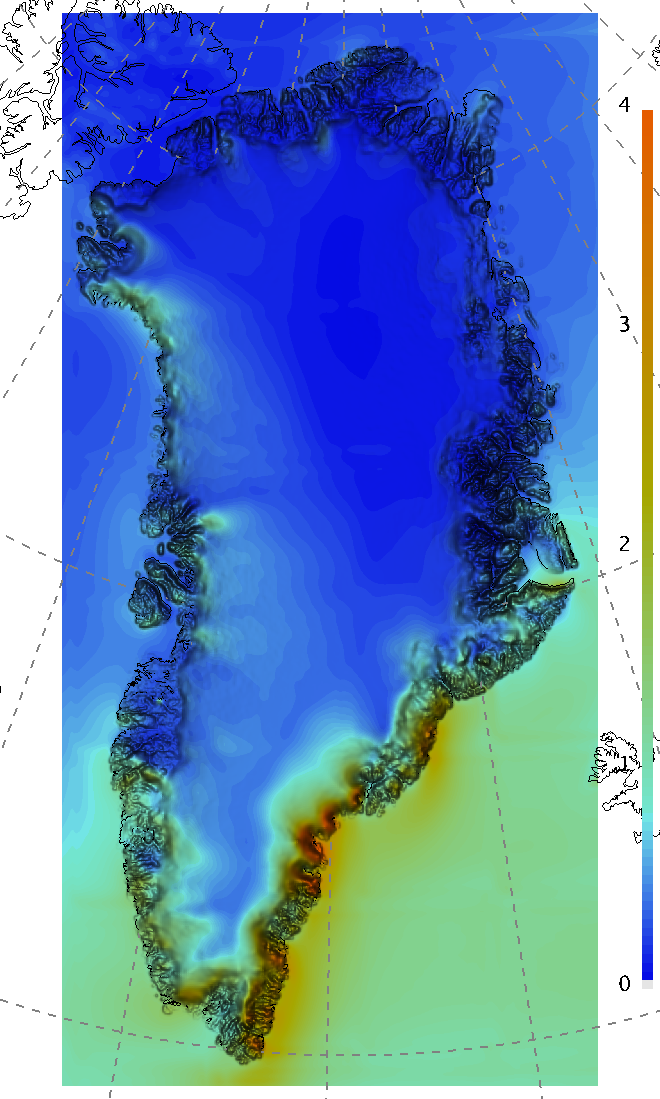
\includegraphics[width=2.0in,keepaspectratio=true]{sr-greenland-prcp}}
\caption{The input present-day ice thickness (left; m), bedrock elevation (center; m), and present-day precipitation (right; m $\text{a}^{-1}$ ice equivalent) for SeaRISE-Greenland.  These are fields \texttt{thk}, \texttt{topg}, and \texttt{precipitation}, respectively, in file \texttt{pism_Greenland_5km_v1.1.nc} produced by running \texttt{preprocess.sh}.}
\label{fig:sr-input}
\end{figure}


\subsection{Run PISM}   \label{subsect:runscript}  Like many Unix programs, PISM allows many command-line options.  Because PISM handles a wide variety of ice sheet, shelf, and glacier sub-models and configurations, the list of possible command-line options is long; see sections \ref{sec:boot} through \ref{sec:practical-usage} of this manual.  Therefore, in practice, one often builds scripts to run PISM with the correct options.

Our script is called ``\texttt{spinup.sh}''.  Initializing ice sheets can be done by computing approximate steady states with constant boundary data, or, in some cases, by integrating paleo-climatic and long-time-scale information to build a model for the present state of the ice sheet.  Both of these possibilities are illustrated in the \texttt{spinup.sh} script.  The spin-up stage may even require the most processor-hours, compared to a follow-on ``experiment'' or ``forecast'' stages.

We are ready to run PISM.  To see what can be done with the script, read the usage message it produces:
\begin{verbatim}
$ ./spinup.sh
\end{verbatim}
The simplest spin-up approach is to use a ``constant-climate'' model.  We take this approach here, first.

To see a more detailed view of the run we will do first, try:
\begin{verbatim}
$ PISM_DO=echo ./spinup.sh 4 const 10000 20 sia g20km_10ka.nc
\end{verbatim}
Setting the environment variable \texttt{PISM_DO} in this way tells \texttt{spinup.sh} just to print out the commands it is about to run, not do them.  The ``proposed'' run looks like this:
\small
\begin{verbatim}
mpiexec -n 4 pismr -boot_file pism_Greenland_5km_v1.1.nc -Mx 76 -My 141 \
  -Mz 101 -Mbz 11 -z_spacing equal -Lz 4000 -Lbz 2000 -skip -skip_max 10 \
  -ys -10000 -ye 0 -surface given -surface_given_file pism_Greenland_5km_v1.1.nc \
  -ocean_kill pism_Greenland_5km_v1.1.nc -sia_e 3.0 \
  -ts_file ts_g20km_10ka.nc -ts_times -10000:yearly:0 \
  -extra_file ex_g20km_10ka.nc -extra_times -10000:100:0 \
  -extra_vars diffusivity,temppabase,tempicethk_basal,bmelt,tillwat,csurf,mask,thk,topg,usurf \
  -o g20km_10ka.nc
\end{verbatim}
\normalsize
Let's briefly deconstruct this run.

At the front is ``\texttt{mpiexec -n 4 pismr}''.  This means that the PISM executable \texttt{pismr} is run in parallel on four processes (e.g.~cores).  Though this example assumes you have a workstation or laptop with at least 4 cores, it will work with 1 to 100 processors, with reasonably good scaling in speed.  (Scaling can be good with far more processors if we run at higher spatial resolution.)  The executable name ``\texttt{pismr}'' stands for the standard ``run'' mode of PISM, in contrast to other, specialized modes described later (e.g.~in sections \ref{sec:verif} and \ref{sec:simp}).

Next, the proposed run uses option \texttt{-boot_file} to start the run by ``bootstrapping,'' a term describes the creation, by heuristics and highly-simplified models, of the complete initial conditions required for a deterministic, time-dependent ice dynamics model.  Then the options describe a $76\times 141$ point grid in the horizontal, which gives 20 km grid spacing in both directions.  Then there are choices about the vertical extent and resolution of the computational grid; more on those later.  After that we see a description of the time-axis, with a start and end time given: ``\texttt{-ys -10000 -ye 0}''.

Then we get the instructions that tell PISM to read the upper surface boundary conditions (i.e.~climate) from a file: ``\texttt{-surface given -surface_given_file pism_Greenland_5km_v1.1.nc}''.  For more on these choices, see subsection \ref{sec:climate-inputs}, and also the PDF PISM Climate Forcing Manual.

Following that there are longish options describing the fields we want as output, including scalar time series (``\texttt{-ts_file ts_g20km_10ka.nc -ts_times -10000:yearly:0}''; see section \ref{sec:practical-usage}), time- and space-dependent fields (``\texttt{-extra_file ...}''; again see section \ref{sec:practical-usage}), and finally the named output file (``\texttt{-o g20km_10ka.nc}'').

Now let's actually get the run going:
\begin{verbatim}
$ ./spinup.sh 4 const 10000 20 sia g20km_10ka.nc &> out.g20km_10ka &
\end{verbatim}
\noindent Because we have re-directed the text output, PISM will show what it is doing in the text file \texttt{out.g20km_10ka} as it runs in the background.  Using \texttt{less} is a good way to watch such a growing text-output file.

% FIXME: replace this?  Soon after that some climatic boundary conditions sample results will appear in \texttt{g20km_climate-500a.nc}.  Such output is effectively a movie of the stored and modeled climatic inputs provided to our ice dynamics model, including the results from surface models like the above-mentioned PDD model for surface mass balance.  This is a convenient way to, early in the modeling process, look at the critical surface mass balance and surface temperature inputs to the ice dynamics.


\subsection{Watching the spin-up}  \label{subsect:spinupsketch}  The next paragraphs describe what happens and what files are produced by the run which is underway.  We believe that the modeling choices represented here are reasonable, but they are not the only way to do it.  The user is encouraged to experiment; that is the point of a model!

FIXME FROM HERE:  After the completion of the first 100 model year run (\texttt{g20km_pre100.nc}), we then work to generate a more-physical enthalpy (i.e.~temperature and liquid fraction) field in which the modeled ice internal energy, its temperature, its softness, its stored basal water, and its basal melt rate are all in better balance with the ice sheet geometry and the simultaneously evolving flow velocity field.  Note the velocity advects the ice properties, especially enthalpy and thus ice softness.

The upper and lower surfaces of this modeled ice are held fixed at this stage.  The upper surface is held fixed by the option \texttt{-no_mass}, while the lower surface is held fixed in the sense that we do not yet apply a bed deformation model.  The resulting enthalpy field is in approximate equilibrium with a velocity field for which the surface kinematical equation \cite{Fowler} is unfortunately \emph{not} satisfied.  Also there is no sliding at this stage because good sliding requires good basal strength which requires good basal melt rates; these improve significantly as this no-sliding run evolves.

We sometimes call this early stage ``pre-spin-up'', a stage which follows on ``bootstrapping'' and comes before the classical paleo-climatic data-using ``spin-up''.  This ``pre-spin-up'' stage goes for 50,000 model years and yields the file \texttt{g20km_steady.nc} at the end.  Along the way the file \texttt{ex_g20km_steady.nc} is updated at every 500 model years, and it can be used to evaluate the degree to which we have reached a thermomechanically-coupled steady state.


\begin{figure}[ht]
\centering
%  temppabase from last time in ex_g10km_steady.nc and driving stress taud from g10km_SIA.nc
\mbox{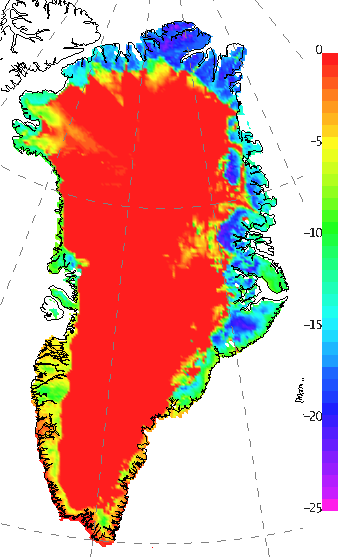
\includegraphics[width=2.0in,keepaspectratio=true]{temppabase}
  \qquad 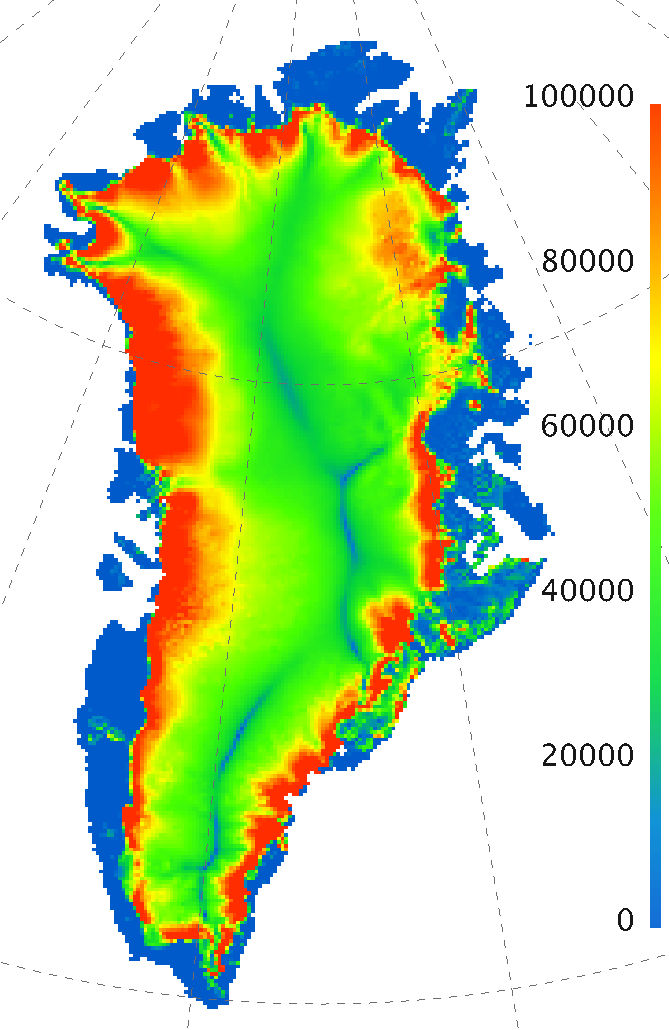
\includegraphics[width=2.1in,keepaspectratio=true]{taud}}
\caption{Part of the model state at the beginning of paleo-climate-modeling ice sheet spin-up, in file \texttt{g20km_steady.nc} from running \texttt{spinup.sh}.  Left: pressure-adjusted basal temperature ($\phantom{|}^\circ$C; field \texttt{temp_pa}).  Right: driving stress magnitude $\rho g H |\grad h|$ (Pa; field \texttt{taud_mag}).}
\label{fig:sr-spinstart}
\end{figure}

The resulting model state in \texttt{g20km_steady.nc} is our model for the state of the Greenland ice sheet at the beginning of the paleo-climate record provided in the SeaRISE data set, namely 125,000 B.P.  There is, obviously, great uncertainty in this model for the distant past of the Greenland ice sheet.  Two views of the 10\,km model grid version of this state are in Figure \ref{fig:sr-spinstart}.

\begin{figure}[ht]
\centering
%  thk, cbase, csurf from g10km_0.nc
\mbox{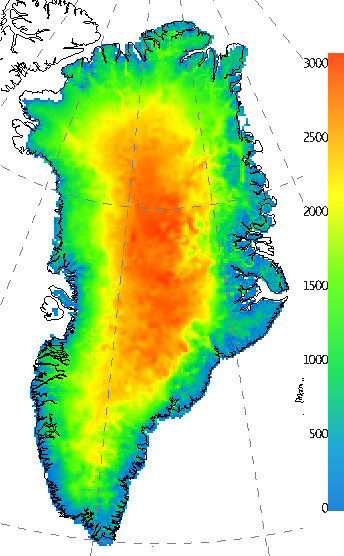
\includegraphics[width=2.in,keepaspectratio=true]{thk}
  \qquad 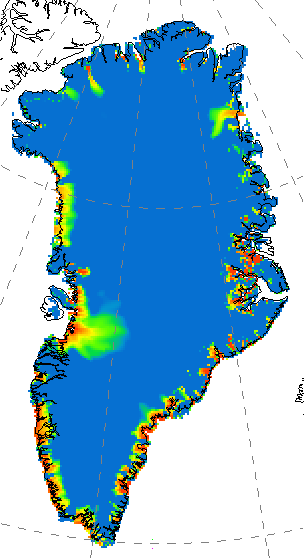
\includegraphics[width=2.in,keepaspectratio=true]{cbase}
  \qquad 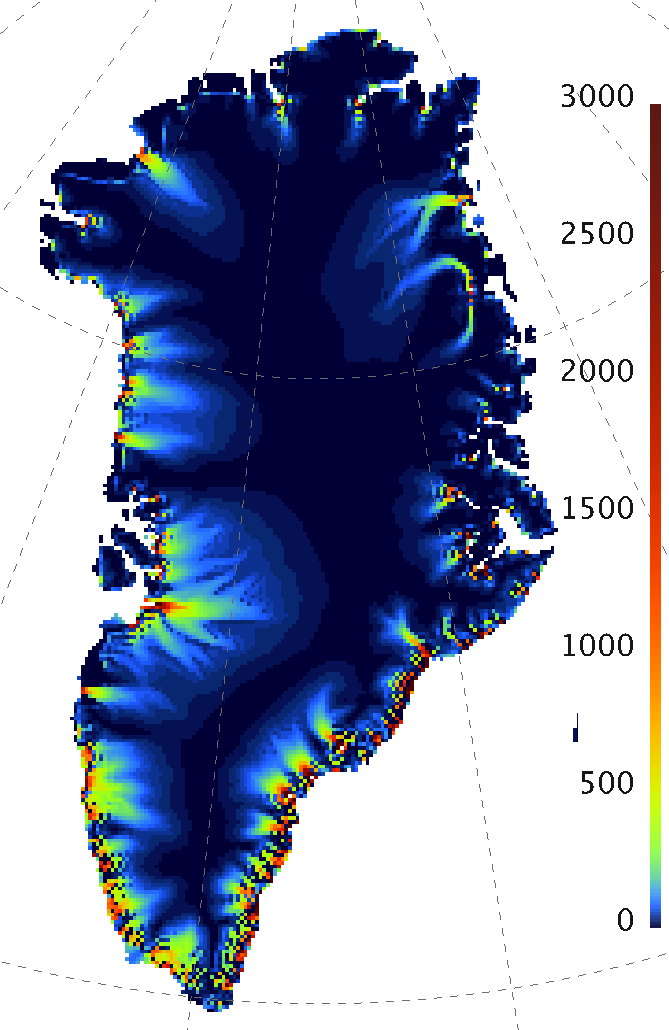
\includegraphics[width=2.in,keepaspectratio=true]{csurf}}
\caption{Model for the present-day Greenland ice sheet, based on spin-up over 125,000 model years using paleo-climate forcing.  Left: ice thickness (m).  Center: basal sliding speed (m/a).  Right: surface speed (m/a).  These are fields \texttt{thk}, \texttt{cbase}, and \texttt{csurf} from file \texttt{g10km_0.nc}.}
\label{fig:sr-spindone-map}
\end{figure}

The actual paleo-climate-driven spin-up starts from model state \texttt{g20km_steady.nc}.  We turn on three new mechanisms, climatic forcing, bed deformation, and improved stress balance.  There are two forms of climatic forcing. First, temperature offsets from GRIP core data affect the snow energy balance and thus rates of melting and runoff; the model is a simple temperature-index scheme described at the SeaRISE website.  Thereby the surface mass balance varies over time; in warm periods there is more marginal ablation.  Additionally, sea levels from the SPECMAP cores affects which ice is floating.

Significantly, we start using a more complete ice dynamics model with sliding controlled by a membrane stress balance, the SIA+SSA hybrid model described in section \ref{sec:dynamics}.  This is turned on with option ``\texttt{-ssa_sliding}''.  Also, we turn on a bed deformation model; the option is ``\texttt{-bed_def lc}''.  These options are discussed in section \ref{sec:modeling-dynamics}.  The command itself (do \verb|PISM_DO=echo ./spinup.sh 8| to see) is
\small
\begin{verbatim}
mpiexec -n 8 pismr -config_override searise_config.nc -climatic_mass_balance_cumulative -skip -skip_max 10 \
  -i g20km_steady.nc -ssa_sliding -topg_to_phi 5.0,20.0,-300.0,700.0 -bed_def lc \
  -atmosphere searise_greenland,delta_T -surface pdd -paleo_precip pism_dT.nc \
  -atmosphere_delta_T_file pism_dT.nc \
  -ocean constant,delta_SL -ocean_delta_SL_file pism_dSL.nc -ocean_kill pism_Greenland_5km_v1.1.nc \
  -ts_file ts_g20km_m5000a.nc -ts_times -125000:yearly:-5000 -extra_file ex_g20km_m5000a.nc \
  -extra_vars ... -extra_times -125000:500:-5000 -ys -125000 -ye -5000 -o g20km_m5000a.nc
\end{verbatim}
\normalsize
but where the full list \verb|-extra_vars| is suppressed.  It uses option \verb|-i| for its input file \verb|g20km_steady.nc|, which is a PISM output file containing the grid information; contrast this with the earlier run which had options \verb|-boot_file| and specified a grid.   (A grid specification uses options \verb|-Mx|, \verb|-My|, \verb|-Mz|, etc.; see subsection \ref{subsect:grid}.)  This run command illustrates that PISM allows a great deal of command-line control, which is a desirable feature, but it also means in practice that most PISM modeling is done using shell scripts to run executables, as here.

This run goes from the SeaRISE-Greenland start time of -125,000 years to -5,000 years.  In this period, diagnostic outputs are written into \texttt{ex_g20km_m5000a.nc} at every 500 model years, and scalar time series including total ice volume are written into \texttt{ts_g20km_m5000a.nc} at every model year.  At the end of this period of the spinup we get the model state file \texttt{g20km_m5000a.nc}.  After that, a final run continues on the same grid from -5,000 years to present day, producing \texttt{g20km_0.nc}.  A variation on this last 5,000 model years run is put in \texttt{g20km_0_ftt.nc}.



The spun-up states \texttt{g20km_0.nc} or \texttt{g20km_0_ftt.nc} is intended to be a model for the Greenland ice sheet at the present day, and thus a basis on which to explore future ice sheet behavior.  If you run \texttt{./spinup N 2} then all of this is done on a 10\,km grid.  Figure \ref{fig:sr-spindone-map} shows some fields from the 10\,km model grid version of this present-day state.  The ice sheet thickness and surface velocity can be compared to present-day observations \cite{BKAJS}, and parameter dependences in the spin-up process should be explored.

Over the course of the spin-up we have saved the modeled ice volume in ``time-series'' NetCDF files.  This important model output can be viewed by
\begin{verbatim}
$ ncview ts_g20km_m5000a.nc ts_g20km_0.nc
\end{verbatim}
\noindent Figure \ref{fig:sr-spindone-ivolboth} shows this ice volume time series for the whole spin-up.  We see the modeled volatility of ice volume in the late ``Eemian'' period, between -120,000 and -115,000 BPE in the SeaRISE version of the GRIP temperature data.  We also see that the result \emph{does} depend on resolution.  Higher resolution grids allow the model to better resolve the flux through outlet glaciers especially, which are topographically-controlled, and such an effect explains the greater Eemian volume loss in the above 10\,km time series.  See the later examples in this manual for more on high resolution modeling.

\begin{figure}[ht]
\centering

\includegraphics[width=4.5in,keepaspectratio=true]{ivolboth}
\caption{Time series of modeled ice sheet volume on 20km and 10km grids.}
\label{fig:sr-spindone-ivolboth}
\end{figure}

%from PISM0.4:  On an 8 core workstation the total run time for the complete 20\,km spin-up, which models 125,000 model years with ``full physics'' of the polythermal SIA+SSA hybrid type (section \ref{sec:dynamics}) is about 5 wall clock hours or 40 processor-hours.  For the same machine, the complete 10\,km spin-up used about 660 processor-hours, thus several wall-clock days.

On an the total run time for the complete 20\,km spin-up, which models 125,000 model years with ``full physics'' of the polythermal SIA+SSA hybrid type (section \ref{sec:dynamics}) is about 290 processor-hours.  The complete 10\,km spin-up used about 6131 processor-hours.

If done without membrane stresses (i.e.~non-sliding SIA only) these computational times are significantly reduced.  The polythermal versus ``cold'' energy-conservation choice corresponds to no performance difference of consequence.


\subsection{Going forward}  \label{subsect:forecastcaution}  In the same \verb|examples/searise-greenland| directory is a script \verb|experiments.sh|.  This does a suite of runs for 500 years into the future for the SeaRISE assessment, initializing from the above-computed modeled present-day state.  The first run is a ``control''  run assuming steady climate for the entire period.  Other runs perform the experiments described at \url{http://websrv.cs.umt.edu/isis/index.php/Category_1:_Whole_Ice_Sheet}.  Some runs use the AR4 climate forcing files which were produced when you ran \texttt{preprocess.sh}.  Once these runs are completed there are postprocessing scripts which primarily adjust metadata to match the standardizations used for the SeaRISE assessment.

Please run \verb|experiments.sh| and the postprocessing scripts, play with them, and modify them, but remember that we include these scripts for demonstration purposes.

Because real ice sheets, and ice sheet models too, have a ``memory'' of past climates, the results strongly depend on the nature of the spin-up process which preceded this ``forecast'' run.  Therefore, as already noted, it is critical to evaluate the quality of the spunup state, for example using present-day observations of surface velocity \cite{AschwandenAdalgeirsdottirKhroulev}, and other observations including ice temperature in ice bore-holes.  Critical thinking about a broad range of modeling hypotheses is prerequisite to building models of future behavior.


\subsection{Handling NetCDF files}\label{subsect:nctoolsintro}  PISM takes one or more NetCDF files as input, then it does some computation, and then it produces one or more NetCDF files as output.  Usually, other tools help to extract meaning from these NetCDF files, and yet more tools help with creating PISM input files or post-processing PISM output files.

Table \ref{tab:NetCDFview} lists such tools.  We frequently use \texttt{ncview}, ``\texttt{ncdump -h}'', and NCO for quick visualization, metadata examination, and command-line manipulation, respectively.  Visualization tools IDV and PyNGL are especially useful.  

To use CDO on PISM files, first run the script \texttt{nc2cdo.py}, from the \texttt{util/} PISM directory, on the file.  This fixes the metadata so that CDO will understand the mapping.

Regarding the creation of input files for PISM, see the section \ref{sec:bootstrapping-format} and table \ref{tab:modelhierarchy} for ideas about the data necessary for modeling.

\newcommand{\netcdftool}[1]{#1\index{NetCDF!tools!#1}}
\begin{table}[ht]
\centering
\small
\begin{tabular}{llp{0.4\linewidth}}
  \toprule
  \textbf{Tool} & \textbf{Site} & \textbf{Function} \\
  \midrule
  & \url{www.unidata.ucar.edu/software/netcdf/} & root for NetCDF information \\
  \midrule
  \netcdftool{\texttt{ncdump}} & \emph{included with any NetCDF distribution} & dump binary NetCDF as \texttt{.cdl} (text) file \\
  \netcdftool{\texttt{ncgen}} & \emph{included with any NetCDF distribution} & convert \texttt{.cdl} file to binary NetCDF \\
  \midrule
  \netcdftool{CDO} & \url{http://code.zmaw.de/projects/cdo} & = Climate Data Operators; command-line tools, including conservative re-mapping \\
  \netcdftool{IDV} & \url{http://www.unidata.ucar.edu/software/idv/} & more complete visualization \\
  \netcdftool{NCO}\index{NCO (NetCDF Operators)} & \url{http://nco.sourceforge.net/} & = NetCDF Operators; command-line tools\\
  \netcdftool{NCL} &  \url{http://www.ncl.ucar.edu} & = NCAR Command Language\\
  \netcdftool{\texttt{ncview}} & \href{http://meteora.ucsd.edu/~pierce/ncview_home_page.html}{\texttt{meteora.ucsd.edu/$\sim$pierce/ncview_home_page.html}} & quick graphical view \\
  \netcdftool{PyNGL} &  \url{http://www.pyngl.ucar.edu} & Python version of NCL\\
  \bottomrule
\end{tabular}
\normalsize
\caption{A selection of tools for viewing and modifying NetCDF files.}
\label{tab:NetCDFview}
\end{table}


%%% Local Variables: 
%%% mode: latex
%%% TeX-master: "manual"
%%% End: 


% LocalWords:  metadata SPECMAP paleo html IDV
